\section{Introduction}

Robot dexterity is critically important for robots working alongside people and for robots working in human spaces.    Robots must be able to manipulate human objects and use tools made for people in order to assist people in performing tasks from mission critical to everyday.   

\begin{figure}
\begin{center}
{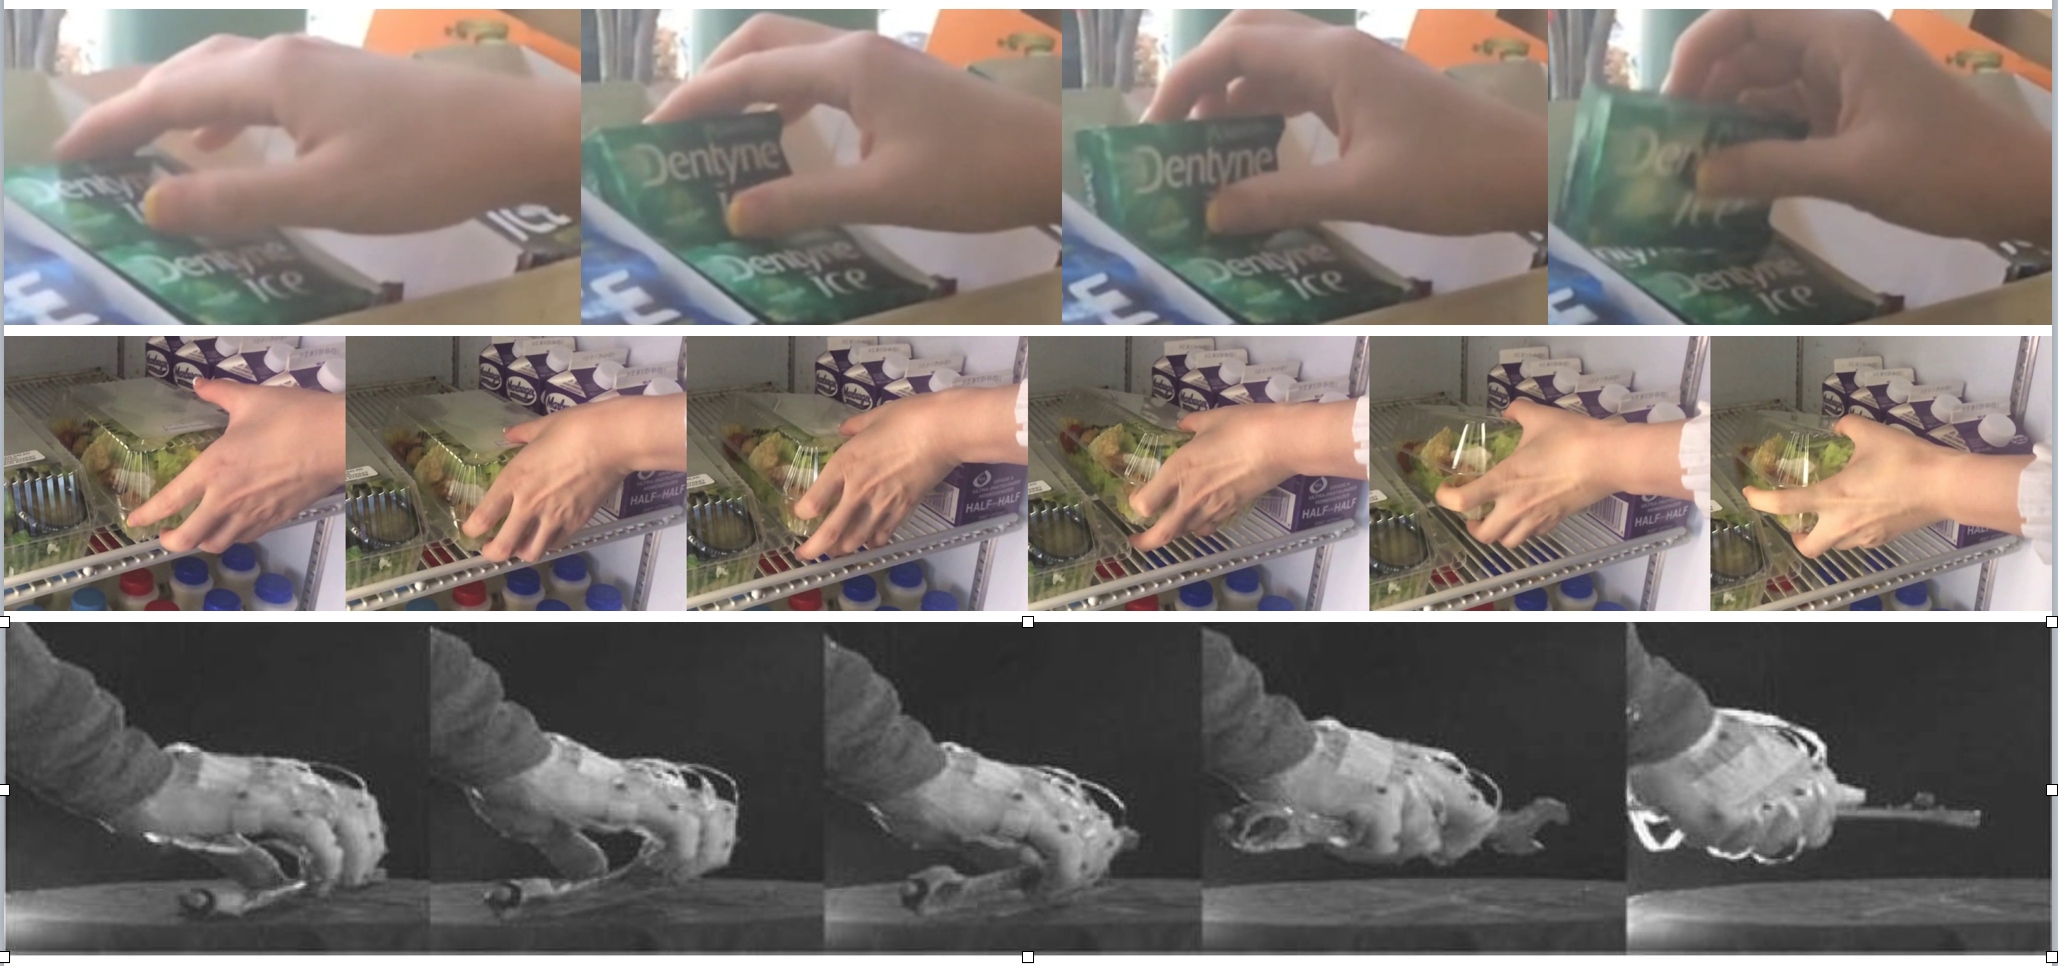
\includegraphics[height=1.7in]{./figs/acquireObject.png}}
{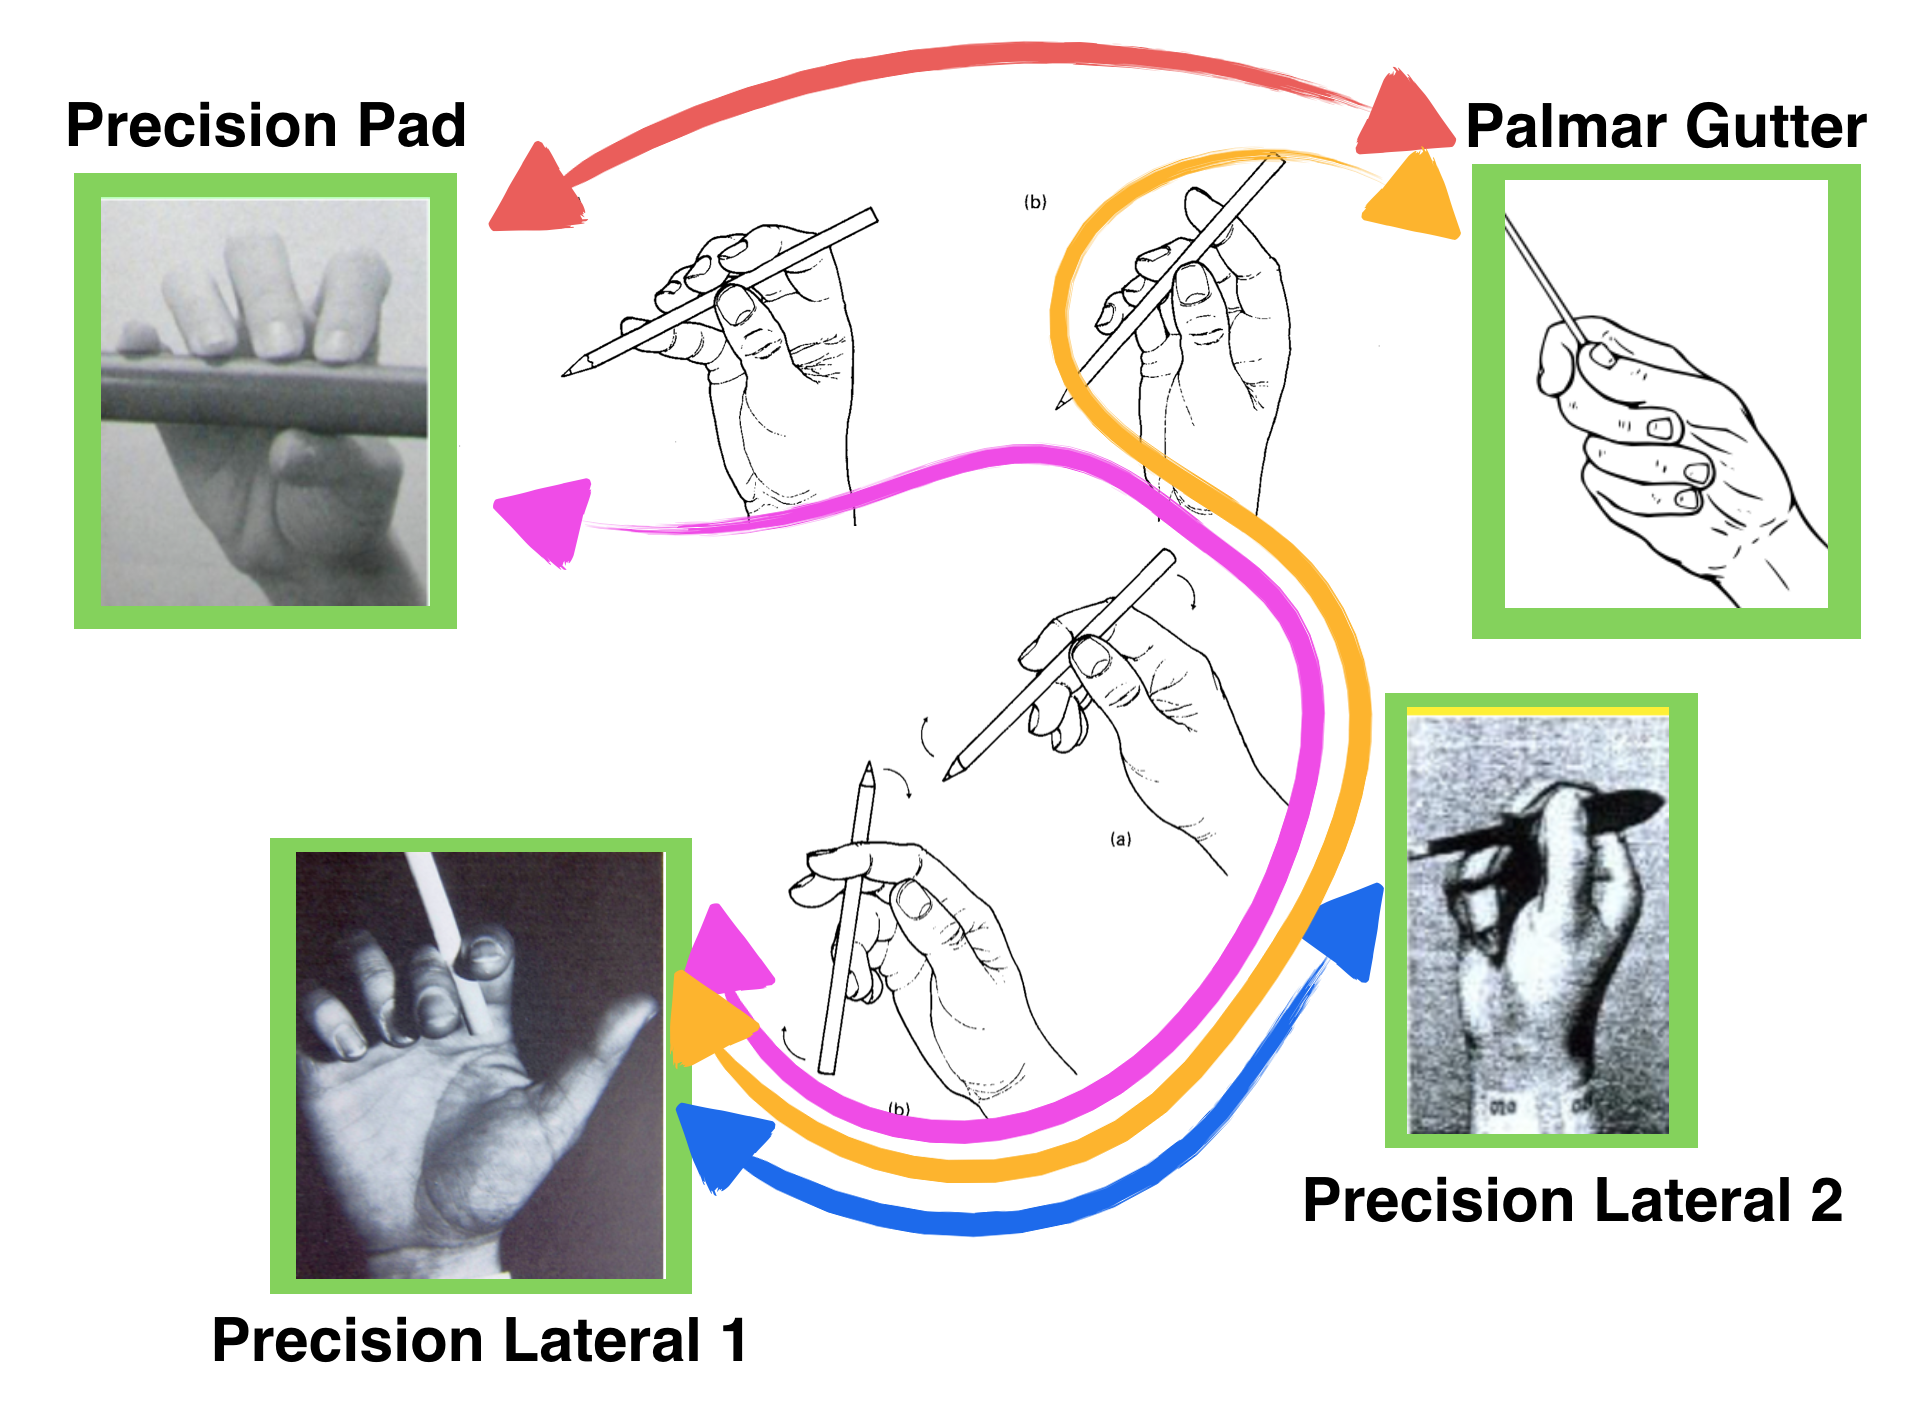
\includegraphics[height=1.7in]{./figs/smallGraspNet.png}}
\end{center}
\vspace*{-0.2in}
\caption[]{\small We propose to develop the underlying analysis techniques and mechanism optimization approaches to enable us (and others) to design  robot hands from the ground up to perform robustly dexterous manipulation tasks such as these.}
\label{DexterousExamples}
\end{figure}

Unfortunately, despite decades of development, dexterous manipulation has remained elusive.   Robot hands cannot lift a wrench in a pinch grasp and slide it into a secure grasp for use with ease.   Robot hands cannot handle a pair of pliers with competence.   Even the simple task of grasping and turning a lever or knob can be a challenge;   compare to the variety of modes of the ``twist" action shown in Figure \ref{GraspNet}.   Our view is that robots fail in these tasks in large part because no one has designed a robot hand from the ground up to be robustly competent at exactly these kinds of manipulations.

The 2013 Robotics Roadmap \cite{christensen2009roadmap} states:
\begin{quotation}
{\small \it
Robot arms and hands will eventually out-perform human hands. This is already true in terms of speed and strength. However, human hands still out-perform their robotic counterparts in tasks requiring dexterous manipulation. This is due to gaps in key technology areas, especially perception, robust high fidelity sensing, and planning and control. The roadmap for human-like dexterous manipulation consists of the following milestones:
\begin{itemize}
	\item 5 years: Low-complexity hands with small numbers of independent joints will be capable of robust whole-hand grasp acquisition.
	\item 10 years: Medium-complexity hands with ten or more independent joints and novel mechanisms and actuators will be capable of whole-hand grasp acquisition and limited dexterous manipulation.
	\item 15 years: High-complexity hands with tactile array densities, approaching that of humans and with superior dynamic performance, will be capable of robust whole-hand grasp acquisition and dexterous manipulation of objects found in manufacturing environments used by human workers.
\end{itemize}}
\end{quotation}
Dexterous manipulation is not mentioned for the 5 year milestone.   Dexterity is expected in limited form at 10 years, and approaching human levels in 15 years.

{\it We propose to enable dexterity at the 5 year mark by designing robot hands from the ground up to do the kinds of dexterous manipulation tasks we see in Figure~\ref{DexterousExamples}}.   This figure shows several examples of dexterously acquiring objects into the hand, as well as a collection of manipulation actions to move between four different grasps.  Later figures have other examples.

There are many very excellent research groups working on the critical areas of sensing, planning, and control.   Our approach is orthogonal and complementary to these efforts.    We aim to reduce the load on sensing, planning and control by designing the mechanism to be as favorable to the intended task set as possible by developing new analysis and design tools for optimizing the robot hand to make dexterous manipulation easier from the start.

This is a {\bf high risk / high reward proposal}.   The risk derives from the fact that dexterous manipulation is indeed complex.   However, we observe commonalities in how people perform manipulation tasks that indicate sufficient structure to make design optimization feasible.   For the reward, consider the change that can be effected by a robot hand that can manipulate the same objects and tools as its human counterpart in a cooperative task and carry out dexterous actions easily because it was designed to do just that.

Our approach centers around several elements:  {\bf ``Grasp Net" benchmarks} to explore manipulation at its full complexity (Section~\ref{secGraspNet}), {\bf Mechanism design} focused on manipulation tasks (Section \ref{secHandDesign}),  Strategic Placement of {\bf Actuators, Joint Limits, and Compliance} (Section \ref{secManipAnalysis}), and later in the project Strategic consideration of {\bf Sensing} (Section \ref{secQuestions}).

Figure \ref{SimpleExampleResults} shows a very simple robot hand which we developed to illustrate the potential.  Through our design optimization process, we went from a manually designed version that was fiddly and difficult to coordinate to one where the manipulation almost does itself.  A hand designed to do the manipulation tasks in Figure~\ref{DexterousExamples} as robustly as possible will change the landscape in terms of potential robot applications, especially in real-world co-robot applications where humans and robots work together and cooperate to accomplish a goal.


	

